



\documentclass[conference]{IEEEtran}

\usepackage{mathtools}

\usepackage{float}
\usepackage[colorlinks,linkcolor=red,anchorcolor=red,citecolor=red]{hyperref}
\usepackage[pdftex]{graphicx}
\graphicspath{{./graphics/}}
\usepackage{subfigure}
\usepackage{multicol}
\usepackage{paralist}
\usepackage{bm}
\usepackage{amsfonts}
\usepackage{url}
\usepackage{multirow}

\usepackage{color}

\usepackage{stfloats}
\makeatletter
\newif\if@restonecol
\makeatother
\let\algorithm\relax
\let\endalgorithm\relax
\usepackage[linesnumbered,ruled,vlined]{algorithm2e}%[ruled,vlined]{
\usepackage{algpseudocode}
\usepackage{amsmath}
\renewcommand{\algorithmicrequire}{\textbf{Input:}}  % Use Input in the format of Algorithm
\renewcommand{\algorithmicensure}{\textbf{Output:}} % Use Output in the format of Algorithm


\begin{document}

\title{Radio Frequency System of Smartphones}


\author{\IEEEauthorblockN{Yang Guo}
\IEEEauthorblockA{Electronic Information School, Wuhan University, Wuhan, China\\
Student Number: 2016301200360, E-mail: whu\_guoyang@whu.edu.cn}
}






% make the title area
\maketitle

% As a general rule, do not put math, special symbols or citations
% in the abstract
\begin{abstract}
Smart phones represent the leading edge of {\emph{radio frequency(RF)}} personal communications, as well as one of the most challenging of RF product designs. Different corporation brings different set of advanced RF front-end technologies to build a comprehensive mobile platform that is designed to maximize throughput and thermal performance. This is an RF architecture report about an iPhone 7. You can see something interesting.
\end{abstract}

\renewcommand\IEEEkeywordsname{Keywords}
\begin{IEEEkeywords}
iPhone 7, RF architecture, different RFFE solutions.
\end{IEEEkeywords}





\IEEEpeerreviewmaketitle



\section{Introduction}
During the learning process of RF circuits, the most important thing is to combine theory with practice. As we all know, our smartphones contain a complete RF system. It is beneficial for us to have a brief understanding about it. So I searched for information about my iPhone 7 on the Internet and made a report. 

The remainder of this report is organized as follows. We have a general look at RF overall architecture in Section \ref{sec:rfa}. In Section \ref{sec:wsfb} we introduce cellular and wireless about iPhone 7 in detail. Section \ref{sec:rfc} and \ref{sec:orfc} describe RF components on iPhone 7.In Section \ref{sec:dw}, we will see different waveforms in different working modes. Section \ref{sec:orft} shows other RF transceivers chips about smartphones. Finally, the conclusions are laid out in Section \ref{sec:conclusion}.

\section{RF Architecture}\label{sec:rfa}
RF architecture of iPhone 7 adopt Qualcomm RFFE solution. The overall block diagram is illustrated in Fig. \ref{fig:RF_Architecture}.

\begin{figure*}[hb]
	\centering
	\begin{center}
		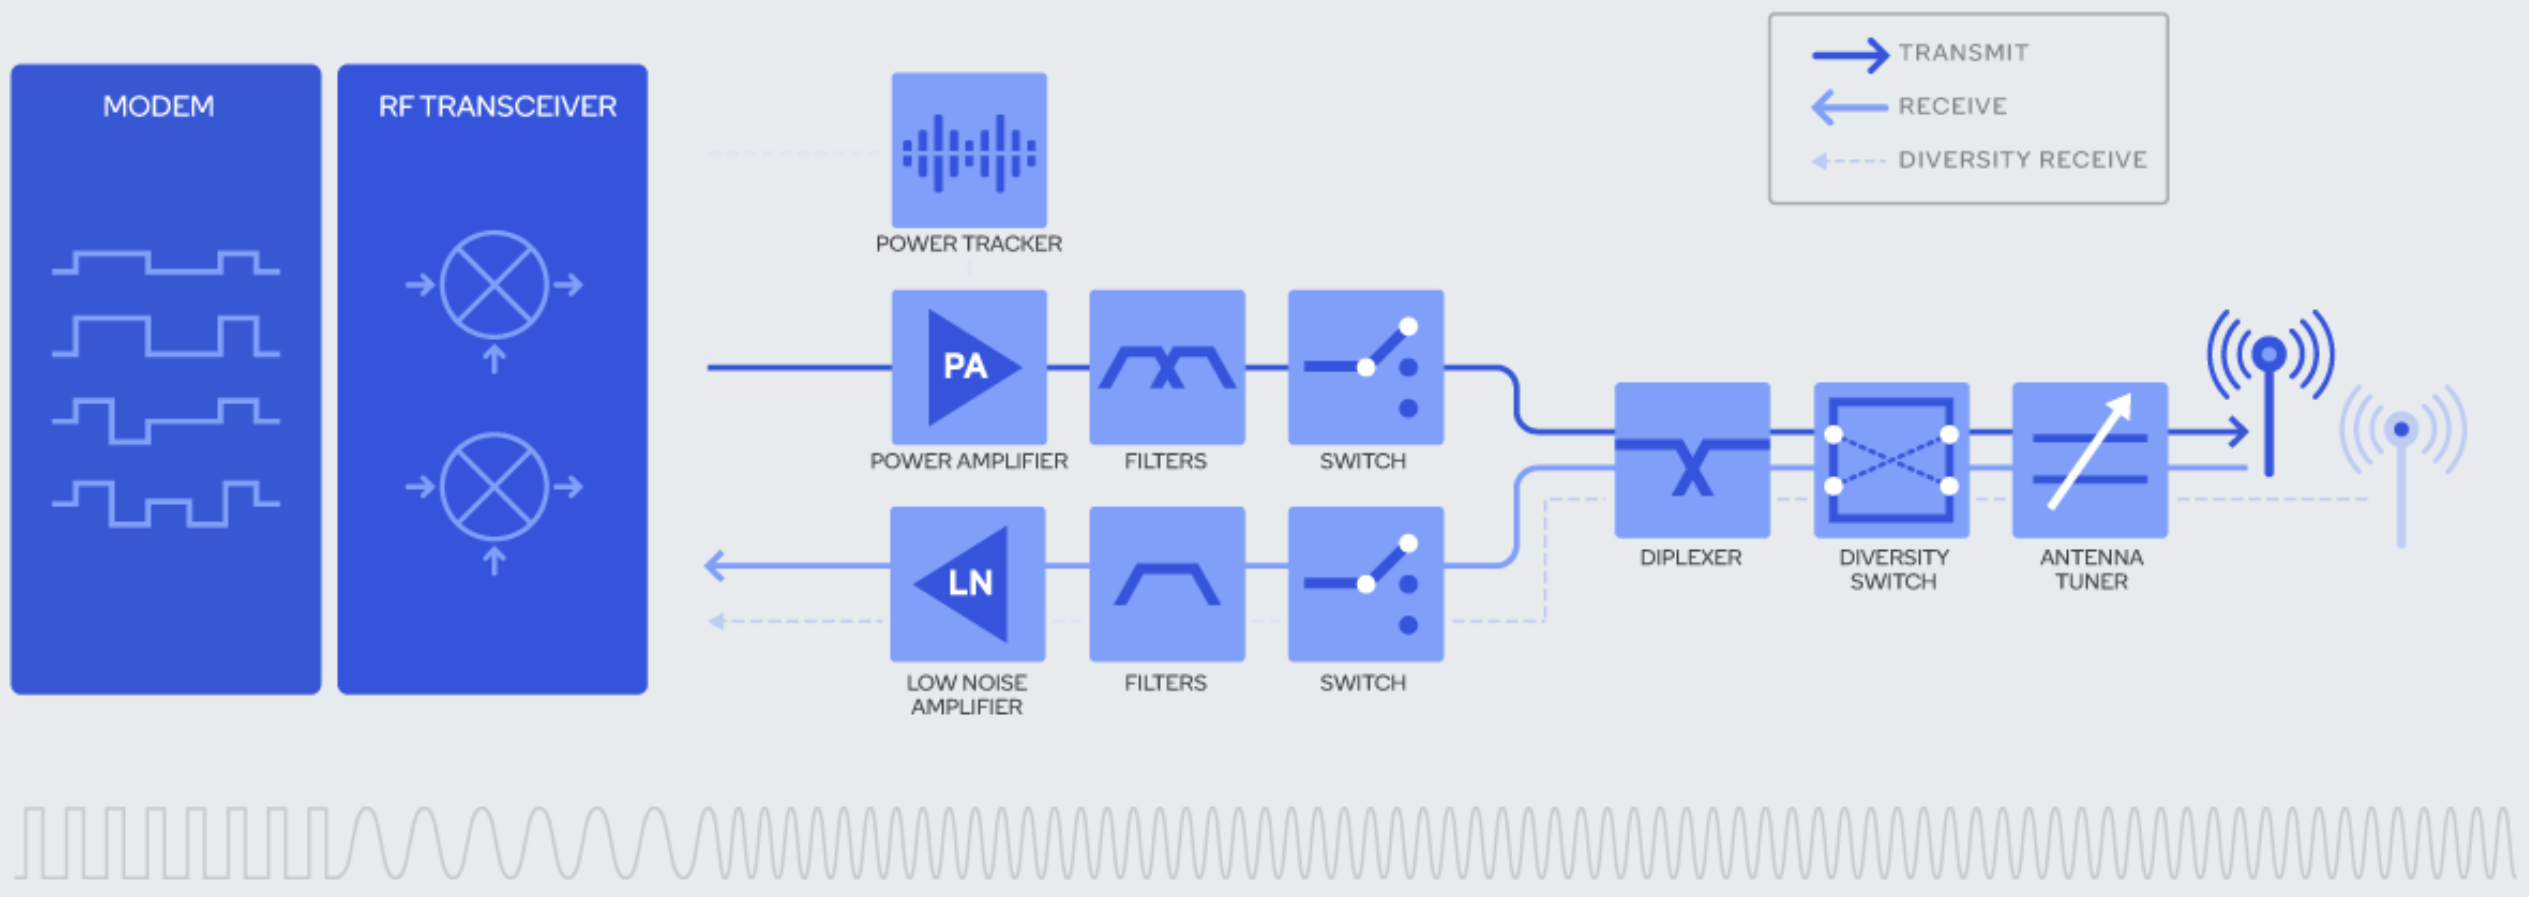
\includegraphics[width=0.92\linewidth]{RF_Architecture}
		\caption{\text{RF Overall Architecture\cite{Qualcomm.org}}} \label{fig:RF_Architecture}	
	\end{center}	
\end{figure*}

From Fig.\ref{fig:RF_Architecture}, we can see that RF overall architecture is consist of several units. We make a brief introduction of them and their functions as follows.
\begin{itemize}
	\item {\bfseries{\emph{Modem}}}: Modems are used to transmit digital information via analog systems. The word "modem" is derived from the term "modulator-demodulator." The essential functions of a modem are to modulate an analog carrier signal to carry digital information; and to demodulate a similar signal so as to decode the digital information from the analog carrier signal\cite{7334868}.
	
	\item {\bfseries{\emph{RF Transceiver}}}: RF transceiver module is used in a particular device where both the transmitter and receiver houses in a single module. Such devices transmit and receives RF signal, so that is named as RF Transceiver. Mostly the position of RF Transceiver module is in between Power amplifier/Low Noise Amplifier and Baseband MODEM in any wireless communication system. Baseband Modem houses, chip sets of several analog or digital modulation techniques and analog to digital conversion or digital to analog conversion chips\cite{6756237},\cite{Exefx.org}.
	
	\item {\bfseries{\emph{Power Amplifier Modules}}}: PA modules bring together multiplexers, filters, RF switches and LNAs to allow highly integrated transmit and receive chains and optimized envelope tracking for premium RF performance while helping to reduce the manufacturer’s time-to-launch\cite{Qualcomm.org}.
	
	\item {\bfseries{\emph{RF Switch and Switch Module}}}: An RF Switch is a device to route high frequency signals through transmission paths. RF and microwave switches are used extensively in microwave test systems for signal routing between instruments and devices under test (DUT)\cite{RFwikipedia.org}. Incorporating a switch into a switch matrix system enables you to route signals from multiple instruments to single or multiple DUTs. This allows multiple tests to be performed with the same setup, eliminating the need for frequent connects and disconnects. The entire testing process can be automated, increasing the throughput in high-volume production environments\cite{DBLP:journals/corr/Truman16}.
	
	\item {\bfseries{\emph{Low Noise Amplifier}}}: Extensive portfolio of integrated and discrete low noise amplifiers (LNAs) to support high performance receive and diversity receive chains in advanced multi-mode, multi-band designs\cite{Qualcomm.org}.
		
	\item {\bfseries{\emph{Filter Products}}}: Electronic filters are circuits which perform signal processing functions, specifically to remove unwanted frequency components from the signal, to enhance wanted ones, or both. Electronic filters can be: passive or active. analog or digital\cite{Electronic_filter.org}. Extensive portfolio of high performance embedded and discrete duplexers, diplexers, extractors, and acoustic filters including SAW, TC-SAW and BAW filters\cite{Qualcomm.org}.
		
	\item {\bfseries{\emph{Antenna Tuner}}}: Antenna Tuner allows the mismatch between the antenna and PA to be minimized. The tuner can operate in open and closed-loop modes. In both the open and closed-loop modes, static (time invariant) mismatch can be addressed, allowing the frequency dependence of the antenna and the RF front-end to be effectively compensated\cite{6546299}.
	
	\item {\bfseries{\emph{Power Trackers}}}: A power tracker is a device that adjusts payload according to the change of power.
	
	\item {\bfseries{\emph{Diversity Receive Module}}}: Diversity receive modules (DRx modules) combine switches, filters and low-noise amplifiers into a module, providing a highly integrated solution for implementing high-order diversity receive paths\cite{Qualcomm.org}.
\end{itemize}

These exist several {\bfseries{\emph{Qualcomm's RF chips}}} on my iPhone's motherboard, which I will talk about in Section \ref{sec:rfc}. So I sought out Fig.\ref{fig:RF_Architecture} on Qualcomm's official website. Just as mentioned above, the Qualcomm RFFE solution includes a comprehensive family of chips: power amplifier modules, power trackers, antenna tuners, RF switches, diversity receive modules, integrated and discrete filters, multiplexers, and extractors. The Qualcomm RFFE solution is designed to address 5G design challenges. 
\section{Working Standard and Frequency Band}\label{sec:wsfb}
The model of my iPhone 7 is A1660. So I visited Apple's official website to check my phone. And I find out its working standard and frequency band as shows in Table. \ref{table:Cellular and Wireless}.
\begin{table}[htbp]
	\centering
	\caption{\text{Cellular and Wireless of iPhone 7 A1660\cite{Apple.org}}}
	\begin{tabular}{c  l}
		\hline \hline
		Working Standard & Frequency Band\label{table:Cellular and Wireless} \\
		\hline
		FDD-LED	&Bands 1, 2, 3, 4, 5, 7, 8, 12, 13, 17, 18,\\ 
		&19, 20, 25, 26, 27, 28, 29, 30\\
		\hline
		TD-LTE	&Bands 38, 39, 40, 41\\
	    \hline
		TD-SCDMA&1900 (F), 2000 (A) \\
		\hline
		CDMA EV-DO Rev. A&800, 1900, 2100 MHz \\
		\hline
		UMTS/HSPA+/DC-HSDPA&850, 900, 1700/2100, 1900, 2100 MHz\\
		\hline
		GSM/EDGE&850, 900, 1800, 1900 MHz\\
		\hline \hline 
	\end{tabular}
\end{table}
\section{Main RF Components}\label{sec:rfc}
Follow the tutorial on the Internet, we can unpack iPhone 7 and get its motherboard as shows in Fig.\ref{fig:board}. I will show several RF components such as {\bfseries{\emph{Modem, LTE Transceiver, RF Transceiver, Diversity Receive, Power Amplifier, Power Management, Filter, Antenna Switch}}} and so on.
\begin{figure}[!ht]
	\centering
	\begin{center}
		\includegraphics*[width=0.8\linewidth]{board}
		\caption{\text{Motherboard of iPhone 7\cite{teardown.org}}}
		\label{fig:board}
	\end{center}
\end{figure}
\subsection{Modem}
The Qualcomm Snapdragon X-series modems are the current line-up of LTE/5G modems. And modem of iPhone 7 is {\bfseries{\emph{Qualcomm MDM9645M}}} as shows in Fig.\ref{fig:modem}.
\begin{figure}[!ht]
	\centering
	\begin{center}
		\includegraphics*[width=0.8\linewidth]{modem}
		\caption{\text{Qualcomm MDM9645M LTE Cat. 12 Modem}}
		\label{fig:modem}
	\end{center}
\end{figure}
\begin{table}[htbp]
	\centering
	\caption{\text{Characteristics of Qualcomm MDM9645M\cite{modem.org}}}
	\begin{tabular}{l | c}
		\hline \hline
		LTE Category (down / up) & 12 / 13\label{table:modem} \\
		\hline
		Peak speeds down (Mb/s)	&600\\ 
		\hline
		Peak speed up (Mb/s)&150\\
		\hline
		LTE/5G Class&630, 660, 820, 821, 636\\
		\hline \hline 
	\end{tabular}
\end{table}

\subsection{LTE Transceiver}
LTE Transceiver of iPhone 7 is {\bfseries{\emph{Qualcomm WTR4905}}} as shows in Fig.\ref{fig:rf}. The red one is Qualcomm WTR4905.
\begin{figure}[!ht]
	\centering
	\begin{center}
		\includegraphics*[width=0.8\linewidth]{rf}
		\caption{\text{LTE and RF Transceiver of iPhone 7}}
		\label{fig:rf}
	\end{center}
\end{figure}

\subsection{RF Transceiver}
RF Transceiver of iPhone 7 is {\bfseries{\emph{Qualcomm WTR3925}}} as shows in Fig.\ref{fig:rf}. The yellow one is Qualcomm WTR3925.

\subsection{Diversity Receive}
Diversity Receives of iPhone 7 are {\bfseries{\emph{Skyworks 13702-20}}} and {\bfseries{\emph{Skyworks 13703-21}}} which are made by Skyworks, an American semiconductor company.

Fig.\ref{fig:Diversity_Receive} shows diversity receives. And the red one is Skyworks 13702-20. The yellow one is Skyworks 13703-21.
\begin{figure}[!ht]
	\centering
	\begin{center}
		\includegraphics*[width=0.8\linewidth]{Diversity_Receive}
		\caption{\text{Diversity Receives of iPhone 7}}
		\label{fig:Diversity_Receive}
	\end{center}
\end{figure}
They have the following features:\cite{Diversity_Receive.org}
\begin{itemize}
	\item RX diversity FEM with seven selectable filters and LNA paths, one Aux path and optional bypass mode 
	\item Low insertion loss thru path 
	\item Integrated SAW filter and discrete LNA gain stage
	\item SAW filters: 791 to 821 MHz
	\item Integrated MIPI interface
	\item Small ($4\times3\times0.7\ mm$)24-lead MCM package(MSL3, $260^{\circ}$C per JEDEC J-STD-020) 
\end{itemize}

\subsection{Filter}
Filter of iPhone 7 is {\bfseries{\emph{Epcos B8856}}}\cite{Ewisetech.org}. It is made by Epcos, a Japanese semiconductor company. The yellow one is Epcos B8856 in Fig.\ref{fig:Power_Management}.

\begin{figure}[!ht]
	\centering
	\begin{center}
		\includegraphics*[width=0.8\linewidth]{pm}
		\caption{\text{Filter and Power Management of iPhone 7}}
		\label{fig:Power_Management}
	\end{center}
\end{figure}

It has the follwing features\cite{B8856.org}.
\begin{itemize}
	\item Low-loss RF filter for mobile telephone WCDMA Band VIII and GSM 900 systems, receive path (RX)
	\item Suitable for diversity applications
	\item Useable passband: 35 MHz
	\item Impedance at input and output 50 $\omega$
	\item Unbalanced to unbalanced operation
	\item FCC/IC/CE certified
\end{itemize}

\subsection{Antenna Switch}
Antenna switch of iPhone 7 is {\bfseries{\emph{Skyworks 13492-21}}}. It has two applications as following:
\begin{itemize}
	\item 2G/3G/4G multimode cellular handsets (LTE, UMTS, CDMA2000,
	EDGE, GSM, TDD-LTE, TD-SCDMA)
	\item Embedded data cards 
\end{itemize}
It has the follwing features\cite{antenna_switch.org}.
\begin{itemize}
	\item Dedicated Band 7 TRX ports: 0.90 dB insertion loss @ 2.7 GHz 
	\item High isolation and linearity 
	\item Broadband frequency range: 0.7 to 2.7 GHz 
	\item Fourteen linear TRX ports
	\item Integrated low- and high-band GSM harmonic filters
	\item External MIPI select pin to enable multiple trigger controls 
	\item Small MCM (24-pin, 2.5 x 3.3 x 0.8 mm) package(MSL3, $260^{\circ}$C per JEDEC J-STD-020) 
\end{itemize}

\subsection{Power Amplifier}
Power Amplifiers of iPhone 7 are {\bfseries{\emph{Avago AFEM-8065}}} and {\bfseries{\emph{Avago AFEM-8055}}} as shows in Fig.\ref{fig:Power_Amplifier}. The red one is Avago AFEM-8055 and the yello one is Avago AFEM-8065.

Avago Technologies AFEM-8065 and AFEM-8055 dual band Front End Module is designed for WLAN applications in both the 2.4GHz and 4.9-5.9 GHz frequency ranges. The FEM is optimized for IEEE 802.11a/b/g/n WLAN applications with dual linear power amplifiers, dual low noise amplifiers, dual Tx/Rx switches, diplexer, Tx and Rx filtering, and direct CMOS compatible control and detect functions. 

By the way, Avago is an American company\cite{Avago.org}.
\begin{figure}[!ht]
	\centering
	\begin{center}
		\includegraphics*[width=0.8\linewidth]{Power_Amplifier}
		\caption{\text{Power Amplifier Transceiver of iPhone 7}}
		\label{fig:Power_Amplifier}
	\end{center}
\end{figure}

They have the following features:\cite{datasheet.org}
\begin{itemize}
	\item 50 $\Omega$ all RF ports
	\item $-10^{\circ}$C to $+85^{\circ}$C operation
	\item Over 17dBm Pout meeting all 802.11 masks
	\item Under 4.0dB NF including switches and filters
	\item Integrated high directivity detector for load insensitive, temp compensated power detection
	\item Integrated bias chokes and DC blocking
	\item +3.3V supply
	\item Small size: $4\times6\times1.2\ mm$
\end{itemize}

\subsection{Power Management}
Power Management of iPhone 7 are {\bfseries{\emph{Dialog 338S00225}}}, {\bfseries{\emph{Qualcomm PMD9645}}} and {\bfseries{\emph{Texas Instruments 65730A0P}}}, as shows in Fig.\ref{fig:Power_Management}. The red one is Qualcomm PMD9645. The green one is Dialog 338S00225. The blue one is Texas Instruments 65730A0P.

I just seek out datasheet of Dialog 338S00225 in Dialog's homepage\cite{dialog.org}, its features was shown below:
\begin{itemize}
	\item 10 Programmable LDOs, High PSRR, 1\% accuracy
	\item 4 Buck Converters (3 with DVS) 0.5 V-2.5 V up to 2 A
	\item Low power Backup Charger 1.1-3.1 V up to 6 mA 32 kHz RTC Oscillator
	\item 10 channel general Purpose ADC with touch screen interface
	\item 16 bit GPIO bus for enhanced wakeup and peripheral control
	\item High voltage boost for white LED driver
	\item 2 Mhz switching frequency avoiding the AM band
	\item Switched DC/USB Charger with power path management
\end{itemize}

By the way, Dialog is a British semiconductor company. It specializes in the production of power management devices.

\subsection{Conclusion of Chips}
Table.\ref{table:Conclusion_of_Chips} is a conclusion of RF chips in my iPhone 7. I list them model, application, manufacturer and country.

\begin{table}[htbp]
	\centering
	\caption{\text{Conclusion of RF Chips}}
	\begin{tabular}{l l l l}
		\hline \hline
		Model & Application & Manufacturer & Country\label{table:Conclusion_of_Chips} \\
		\hline
		MDM9645M&modem&Qualcomm&American\\ 
		\hline
		WTR4905&LTE Transceiver&Qualcomm&American\\
		\hline
		WTR3925&RF Transceiver&Qualcomm&American\\
		\hline
		13702-20&Diversity Receive&Skyworks&American\\
		\hline
		13703-21&Diversity Receive&Skyworks&American\\
		\hline
		B8856&Filter&Epcos&Japan\\
		\hline
		13492-21&Antenna switch&Skyworks&American\\
		\hline
		AFEM-8065&Power Amplifier&Avago&American\\
		\hline
		AFEM-8055&Power Amplifier&Avago&American\\
		\hline
		338S00225&Power Management&Dialog&Britain\\
		\hline
		PMD9645&Power Management&Qualcomm&American\\
		\hline
		65730A0P&Power Management&TI&American\\
		\hline
		339S00199&Wi-Fi and Bluetooth&Murata&Japan\\
		\hline
		67V04&NFC&NXP&Netherlands\\		
		\hline \hline 
	\end{tabular}
\end{table}

\section{Other RF Components}\label{sec:orfc}
These exist other RF components which are different from what I talk about in Section \ref{sec:rfc}. And they have several essential functions such as {\bfseries{\emph{NFC}}}, {\bfseries{\emph{Wi-Fi}}}, {\bfseries{\emph{Bluetooth}}} and so on.

\subsection{Wi-Fi and Bluetooth}
You can see from Fig.\ref{fig:wifi_bluetooth_NFC}, the yellow one is {\bfseries{\emph{Murata 339S00199}}}. It is very important because my phone can not use Wi-Fi and bluetooth without it. 
\begin{figure}[!ht]
	\centering
	\begin{center}
		\includegraphics*[width=0.8\linewidth]{wifi_bluetooth_NFC}
		\caption{\text{Other RF Components of iPhone 7}}
		\label{fig:wifi_bluetooth_NFC}
	\end{center}
\end{figure}

It has the follwing features\cite{wifibluetooth.org}, I find out them on Murata's official website. And Murata is a Japanese semiconductor company.
\begin{itemize}
	\item Supported on NXP i.MX6/7/8 platforms
	\item Various support of Wi-Fi flavors: 802.11b/g/n, 802.11a/b/g/n/ac SISO, 802.11a/b/g/n/ac 2$\times$2 MIMO up to 600Mbps
	\item Cypress official tested release fmac WLAN driver
	\item Advance Bluetooth support (BR/EDR/LE)
	\item Supports all standard profiles from BlueZ
	\item FCC/IC/CE certified
\end{itemize}

\subsection{NFC}
You can see from Fig.\ref{fig:wifi_bluetooth_NFC}, the blue one is {\bfseries{\emph{NXP 67V04}}}. With it, my phone has NFC function. 

It has the following features\cite{NXP.org}, which you can see if you visit NXP Semiconductors's official website\cite{nxp_honepage.org}.
\begin{itemize}
	\item Includes NXP ISO/IEC 14443-A and Innovatron ISO/IEC 14443-B intellectual property licensing rights
	\item Highly integrated demodulator and decoder
	\item Buffered output drivers to connect an antenna with minimum number of external components
	\item Integrated RF level detector
	\item Integrated Polling Loop for automatic device discovery
	\item RF protocols supported(NFCIP-1, NFCIP-2 protocol; – ISO/IEC 14443A, ISO/IEC 14443B PICC mode via host interface; ISO/IEC 14443A, ISO/IEC 14443B PCD designed according to NFC Forum digital protocol T4T platform and ISO-DEP; FeliCa PCD; mode MIFARE Classic PCD encryption mechanism; NFC Forum tag 1 to 4; ISO/IEC 15693/ICODE VCD mode)
	\item Supported host interfaces(NCI protocol interface according to NFC Forum standardization; I2C-bus High-speed mode)
	\item Integrated power management unit
	\item Automatic wake-up via RF field, internal timer and I2C-bus interface	
\end{itemize}

\subsection{Antenna}
Wi-Fi antenna is shown in Fig.\ref{fig:Wi-Fi_Antenna}. RF antenna is shown in Fig.\ref{fig:RF_Antenna}. And RF antenna flex cable is shown in Fig.\ref{fig:RF_Antenna_Flex_Cable}.
\begin{figure}[!ht]
	\centering
	\begin{center}
		\includegraphics*[width=0.8\linewidth]{antenna1}
		\caption{\text{Wi-Fi Antenna of iPhone 7}}
		\label{fig:Wi-Fi_Antenna}
	\end{center}
\end{figure}

\begin{figure}[htbp]
	\begin{tabular}{c c}
		\begin{minipage}[t]{0.5\linewidth}
			\centering
			\includegraphics*[width=0.8\linewidth]{antenna2}
			\caption{\text{RF Antenna of iPhone 7}}
			\label{fig:RF_Antenna}	
		\end{minipage}
		
		\begin{minipage}[t]{0.5\linewidth}
			\centering
			\includegraphics*[width=0.8\linewidth]{antenna3}
			\caption{\text{RF Antenna Flex Cable}} 
			\label{fig:RF_Antenna_Flex_Cable}	
		\end{minipage}
	\end{tabular}
\end{figure}

\section{Different Waveforms} \label{sec:dw}
\subsection{FDD}
{\bfseries{\emph{Frequency Division Duplex(FDD)}}} requires two separate wireless communications channels on separate frequencies, one for transmit and the other for received data\cite{6983336}. 

FDD requires two symmetrical segments of spectrum for the uplink and downlink channels. Fig.\ref{fig:FDD} shows FDD waveform.

\begin{figure}[!ht]
	\centering
	\begin{center}
		\includegraphics*[width=0.8\linewidth]{FDD}
		\caption{\text{FDD Waveform}}
		\label{fig:FDD}
	\end{center}
\end{figure}

FDD is used in the following wireless systems:
\begin{itemize}
	\item Microwave (MW) Links
	\item Millimeter Wave (MMW) links
	\item Some 4G/LTE networks (some use TDD)
\end{itemize}

Wireless systems need two separate frequency bands or channels. A sufficient amount of guard band separates the two bands so the transmitter and receiver don't interfere with one another. Good filtering or duplexers and possibly shielding are a must to ensure the transmitter does not desensitize the adjacent receiver.

FDD uses lots of frequency spectrum, though, generally at least twice the spectrum needed by TDD. In addition, there must be adequate spectrum separation between the transmit and receive channels\cite{wireless.org}. These so-called guard bands aren't useable, so they're wasteful. Given the scarcity and expense of spectrum, these are real disadvantages.

FDD also works on a cable where transmit and receive channels are given different parts of the cable spectrum, as in cable TV systems. Again, filters are used to keep the channels separate.

\subsection{TDD}
{\bfseries{\emph{Time Division Duplex(TDD)}}} uses a single frequency band for both transmit and receive. Then it shares that band by assigning alternating time slots to transmit and receive operations. The information to be transmitted—whether it’s voice, video, or computer data—is in serial binary format. Each time slot may be 1 byte long or could be a frame of multiple bytes\cite{6983336}. 

TDD alternates the transmission and reception of station data over time. Time slots may be variable in length. Fig.\ref{fig:TDD} shows TDD waveform.

\begin{figure}[!ht]
	\centering
	\begin{center}
		\includegraphics*[width=0.8\linewidth]{TDD}
		\caption{\text{TDD Waveform}}
		\label{fig:TDD}
	\end{center}
\end{figure}

TDD is used in the following wireless systems:
\begin{itemize}
	\item WiFi Networks
	\item Some 4G/LTE networks (some use FDD)
\end{itemize}

Because of the high-speed nature of the data, the communicating parties cannot tell that the transmissions are intermittent. The transmissions are concurrent rather than simultaneous. For digital voice converted back to analog, no one can tell it is not full duplex.

In some TDD systems, the alternating time slots are of the same duration or have equal DL and UL times. However, the system does not have to be 50/50 symmetrical. The system can be asymmetrical as required\cite{wireless.org}.

There are several comparisons about TDD and FDD in Table.\ref{table:comparisons_about_TDD_and_FDD} that are of particular interest to mobile or cellular telecommunications operators. These are naturally reflected into LTE.

\begin{table*}[htbp]
	\centering
	\caption{\text{Comparison of TDD LTE and FDD LTE Duplex Formats}}\label{table:comparisons_about_TDD_and_FDD}
	\begin{tabular}{c c c}
		\hline \hline
		Parameter & LTE-TDD & LTE-FDD \\
		\hline
		Paired&Does not require paired spectrum as&Requires paired spectrum with sufficient\\
		spectrum&both transmit and receive occur on&frequency separation to allow\\
		&the same channel&simultaneous transmission and reception\\
		\hline
		&Lower cost as no diplexer is needed to &\\
		&isolate the transmitter and receiver. &\\
		Hardware &As cost of the UEs is of major &Diplexer is needed and cost is higher.\\
		cost&importance because of the vast &\\
		&numbers that are produced, this is a &\\
		&key aspect.&\\
		\hline
		&Channel propagation is the same in &Channel characteristics different in both \\
		Channel &both directions which enables &directions as a result of the use of different \\
		reciprocity&transmit and receive to use on set of &frequencies\\
		&parameters&\\
		\hline
		&&UL / DL capacity determined by frequency \\
		&&allocation set out by the regulatory \\
		UL / DL &It is possible to dynamically change&authorities. It is therefore not possible to  \\
		asymmetry&the UL and DL capacity ratio to match &make dynamic changes to match capacity. \\
		&demand&Regulatory changes would normally be \\
		&&required and capacity is normally allocated \\
		&&so that it is the same in either direction.\\
		\hline
		&Guard period required to ensure &\\
		&uplink and downlink transmissions do &\\
		Guard period / &not clash. Large guard period will limit &Guard band required to provide sufficient \\
		guard band&capacity. Larger guard period &isolation between uplink and downlink. \\
		&normally required if distances are &Large guard band does not impact \\
		&increased to accommodate larger &capacity.\\
		&propagation times.&\\
		\hline
		&Discontinuous transmission is &\\
		Discontinuous &required to allow both uplink and &\\
		transmission&downlink transmissions. This can &Continuous transmission is required.\\
		&degrade the performance of the RF &\\
		&power amplifier in the transmitter.&\\
		\hline
		&Base stations need to be &\\
		&synchronised with respect to the &\\
		&uplink and downlink transmission &\\
		Cross slot &times. If neighbouring base stations &Not applicable\\
		interference&use different uplink and downlink &\\
		&assignments and share the same &\\
		&channel, then interference may occur &\\
		&between cells.&\\
		\hline \hline 
	\end{tabular}
\end{table*}

\subsection{OFDM}
In telecommunications, {\bfseries{\emph{orthogonal frequency-division multiplexing (OFDM)}}} is a method of encoding digital data on multiple carrier frequencies. OFDM has developed into a popular scheme for wideband digital communication, used in applications such as digital television and audio broadcasting, DSL internet access, wireless networks, power line networks, and 4G mobile communications.

The main advantage of OFDM over single-carrier schemes is its ability to cope with severe channel conditions (for example, attenuation of high frequencies in a long copper wire, narrowband interference and frequency-selective fading due to multipath) without complex equalization filters. Channel equalization is simplified because OFDM may be viewed as using many slowly modulated narrowband signals rather than one rapidly modulated wideband signal. The low symbol rate makes the use of a guard interval between symbols affordable, making it possible to eliminate intersymbol interference (ISI) and use echoes and time-spreading (in analog television visible as ghosting and blurring, respectively) to achieve a diversity gain, i.e. a signal-to-noise ratio improvement. This mechanism also facilitates the design of single frequency networks (SFNs) where several adjacent transmitters send the same signal simultaneously at the same frequency, as the signals from multiple distant transmitters may be re-combined constructively, sparing interference of a traditional single-carrier system.\cite{Futaki2001Low}

\begin{figure}[htbp]
	\begin{tabular}{c c}
		\begin{minipage}[t]{0.5\linewidth}
			\centering
			\includegraphics*[width=0.8\linewidth]{fdm}
			\caption{\text{FDM Waveform\cite{ofdm.org}}}
			\label{fig:fdm}	
		\end{minipage}
		
		\begin{minipage}[t]{0.5\linewidth}
			\centering
			\includegraphics*[width=0.8\linewidth]{ofdm}
			\caption{\text{OFDM Waveform\cite{ofdm.org}}} 
			\label{fig:ofdm}	
		\end{minipage}
	\end{tabular}
\end{figure}

Fig.\ref{fig:fdm} is the waveform of FDM, and Fig.\ref{fig:ofdm} is the waveform of OFDM. You can see the difference between FDM and OFDM. Obviously, OFDM do not need guard bands.

The process of OFDM is shown in Fig.\ref{fig:processOfOFDM}.
\begin{figure}[!ht]
	\centering
	\begin{center}
		\includegraphics*[width=0.8\linewidth]{ProcessOFDM}
		\caption{\text{The process of OFDM}}
		\label{fig:processOfOFDM}
	\end{center}
\end{figure}

\subsection{Conclusion of Waveform}
\begin{itemize}
	\item You can see comparisons between FDD and TDD in Table.\ref{table:comparisons_about_TDD_and_FDD}.
	\item To tell the truth, OFDM is different from FDD and TDD. It can modulate and multiplex waveform at the same time. You can figure it out from Fig.\ref{fig:FDD}, Fig.\ref{fig:TDD} and Fig.\ref*{fig:processOfOFDM}.
	\item All in all, TDD, FDD, OFDM are widely used in the field of communication.
\end{itemize}

\section{Other RF Transceivers Chips} \label{sec:orft}
Before 2015, Apple’s modem supplier was Qualcomm. But in 2016 when I bought my iPhone 7, Apple has taken a different approach with the decision to source two instead of one baseband chipset suppliers: Qualcomm and Intel.

Apple brought to market two iPhone 7 variants: the GSM/WCDMA/LTE with Intel modem version, and the GSM/CDMA/WCDMA/TD-SCDMA/LTE version with Qualcomm hardware. A new report is highlighting the first performance differences between the iPhone 7 featuring Intel’s modem hardware compared to the iPhone 7 featuring Qualcomm modem hardware.

The report from Cellular Insights\cite{cellularinsights.org} finds that iPhone 7’s equipped with Qualcomm’s MDM9645M modem, which powers the (A1660, A1661) Verizon, Sprint, and SIM-free models, features better cellular performance than the (A1778, A1784) Intel version. Not only that, but the Qualcomm version’s ability to take advantage of Ultra HD Voice has been disabled as well according to the report.

There exit several tests about them two different RF Transceivers Chips what I found in website\cite{cellularinsights.org}.

We tested three unique LTE frequency bands, Band 12(10MHz), Band 4(20MHz), and Band 7(20MHz) in 4$\times$2 MIMO configuration using Transmission Mode 4. While both devices achieved the maximum sustained data rates at the cell center, simulating edge of cell scenarios by reducing power level did cause each iPhone to display two very different personalities.  This allows us to measure RF sensitivity of the device under test while eliminating inter-cell interference and fully controlling the radiated environment. This also allows for high reproducibility and consistency of our tests, and takes into account the performance of the entire RFFE subsystem. 

\subsection{FDD LTE Band 12(10MHz)}
FDD LTE Band 12 is part of the lower 700MHz band plan, covering 15 MHz of contiguous spectrum across three blocks (A, B, C). Most LTE Band 12 deployments are either 5 MHz or 10 MHz wide even though Band 12 can theoretically be deployed up to 15 MHz widths. Coincidentally, LTE Band 12 capable devices are only certified to support up to 10 MHz operation. As opposed to mid and high band spectrum, low frequency such as 700MHz Band 12 can propagate further, penetrate the concrete structure better, and often times is the only LTE layer reaching the device. For this particular reason, high sensitivity of a smartphone receiver is extremely important in challenging signal conditions, and it could make a difference between completing and dropping a VoLTE call.

\begin{figure}[!ht]
	\centering
	\begin{center}
		\includegraphics*[width=0.8\linewidth]{band12}
		\caption{\text{FDD LTE Band 12(10MHz)}}
		\label{fig:band12}
	\end{center}
\end{figure}

Fig.\ref{fig:band12} shows that both iPhone 7 variants perform similarly in ideal conditions. At -96dBm the Intel variant needed to have Transport Block Size adjusted as BLER well exceeded the 2\% threshold. At -105dBm the gap widened to 20\%, and at -108dBm to a whopping 75\%. As a result of such a huge performance delta between the Intel and Qualcomm powered devices, we purchased another A1784 (AT\&T) iPhone 7, in order to eliminate any possibility of a faulty device. The end result was virtually identical. We are hoping that this sudden dip in performance at a specific RSRP value will be further investigated by the engineering and hopefully resolved. At -121dBm, the Intel variant performed more in line with its Qualcomm counterpart. Overall, the average performance delta between the two is in the 30\% range in favor of the Qualcomm variant. 

\subsection{FDD LTE Band 4\&7(20MHz)}
From Fig.\ref{fig:band4} and Fig.\ref{fig:band7}, we find that band 4 is the most commonly deployed LTE spectrum band in North America, while Band 7 deployments are spread across the rest of the globe. Mid and high spectrum bands are used to densify LTE networks and provide incremental capacity. Just like during our Band 12 tests, the iPhone 7 with the Intel modem continues to struggle even at relatively higher RSRP values with unexplainable sharp dips in performance. The gap between the two variants is consistent and north of 30\% again in favor of the Qualcomm variant.
\begin{figure}[!ht]
	\centering
	\begin{center}
		\includegraphics*[width=0.8\linewidth]{band4}
		\caption{\text{FDD LTE Band 4(20MHz)}}
		\label{fig:band4}
	\end{center}
\end{figure}

\begin{figure}[!ht]
	\centering
	\begin{center}
		\includegraphics*[width=0.8\linewidth]{band7}
		\caption{\text{FDD LTE Band 7(20MHz)}} 
		\label{fig:band7}
	\end{center}
\end{figure}

\subsection{Comparison in Bad Conditions}
To put this into perspective, we have compared the edge of cell performance of a few other flagship devices to see how these iPhones compare in less than favorable conditions.

You can check results by observing Fig.\ref{fig:band4comparison}.
\begin{figure}[!ht]
	\centering
	\begin{center}
		\includegraphics*[width=0.8\linewidth]{band4comparison}
		\caption{\text{Comparison in Bad Conditions}}
		\label{fig:band4comparison}
	\end{center}
\end{figure}

\subsection{Summary}
\begin{itemize}
	\item After testing, the conclusion is that the iPhone 7 hardware with the Qualcomm-powered modem has a significant cellular modem performance edge over the Intel variant.
	\item As to why Apple has sourced two baseband suppliers after years of using Qualcomm hardware exclusively, it likely has much to do with broadening its supply chain. In this case, however, it looks like supply chain diversification has resulted in a measurable performance difference between the two models in a lab-controlled environment.
	\item Also worth noting is that the iPhone 7 with the Qualcomm modem is only being sold in China, Japan and in the United States, which means that Apple deemed the Intel version to be good enough for every other territory.
	\item That said, if you’re buying an iPhone 7 for full price in one of the aforementioned territories, then I highly recommend going with the Verizon/Sprint/SIM-free version. Not only does this version seem to perform better from a cellular modem perspective, but it’s also capable of working with most cellular carriers in the US and abroad.	
\end{itemize}

\section{Conclusion}\label{sec:conclusion}
\begin{itemize}
	\item From Table.\ref{table:Conclusion_of_Chips}, we can find that most of RF chips are designed and manufactured by American companies. These companies include {\bfseries{\emph{Qualcomm, Skyworks, Avago, TI}}}. In particular, almost all core chips in RF chips are produced by {\bfseries{\emph{Qualcomm}}}.
	\item From Table.\ref{table:comparisons_about_TDD_and_FDD}, we can draw a conclusion that whether we use {\bfseries{\emph{FDD, TDD or OFDM}}} depends on the actual situation. All of them can multiplex waveform. But only OFDM can modulate and multiplex waveform at the same time.
	\item From Fig.\ref{fig:band4}, \ref{fig:band7} and \ref{fig:band4comparison}, we can see that Qualcomm-powered modem is better than the Intel variant.
	\item What impressed me the most is that our country's {\bfseries{\emph{IC Design Situation}}} is not optimistic, especially after {\bfseries{\emph{ZTE incident}}} last year. This means that as the freshest force nowadays, we must take responsibility to let China have {\bfseries{\emph{a strong "chip"}}}.	  
\end{itemize}


\bibliographystyle{ieeetr}
\bibliography{reference}


% that's all folks
\end{document}

